\documentclass[11pt]{article}

% ---------- Paquetes ----------
\usepackage[utf8]{inputenc}
\usepackage[T1]{fontenc}
\usepackage[margin=2.5cm]{geometry}
\usepackage{amsmath,amssymb}
\usepackage{circuitikz}
\usetikzlibrary{positioning}
\usepackage{enumitem}
\usepackage{booktabs}
\usepackage{array}
\usepackage{tabularx}
\usepackage{graphicx}
\usepackage{xcolor}
\usepackage{titlesec}
\usepackage{hyperref}
\usepackage{fancyhdr}
\usepackage{caption}
\captionsetup{justification=centering, font=it, labelfont={it,bf}}
\captionsetup[figure]{name=Figure}
\captionsetup[table]{name=Table}
\usepackage{float}

\hypersetup{colorlinks=true, linkcolor=blue, urlcolor=blue, citecolor=blue}

\titleformat{\section}{\large\bfseries}{\thesection.}{0.5em}{}
\titleformat{\subsection}{\normalsize\bfseries}{\thesubsection}{0.5em}{}

\pagestyle{fancy}
\fancyhf{}
\fancyhead[L]{Lab. 3 --- Comparators and the Schmitt Trigger}
\fancyhead[R]{\thepage}
\renewcommand{\headrulewidth}{0.4pt}

\setlength{\parindent}{0pt}
\setlength{\parskip}{0.5em}

\newcommand{\blank}[1]{\makebox[#1]{\hrulefill}}

\begin{document}

% =====================================================
% PORTADA / DATOS DEL EQUIPO
% =====================================================
\begin{center}
    {\LARGE \bfseries Lab. 3}\\[0.3em]
    {\Large \itshape Comparators and the Schmitt Trigger}
\end{center}

\vspace{1em}

\noindent Team No. 2

\vspace{0.5em}

\noindent Names:

\begin{tabbing}
\hspace{1cm} \= Jefferson Chinchilla Quesada \hspace{0.3cm} \= 2023152266  \\[0.6cm]
\> Mattio Coghi Quirós \> 2023056023 \\[0.6cm]
\> Nicolás Mena Valerio \> 2022327473
\end{tabbing}

\vspace{1em}
\vspace{1em}

% =====================================================
% REFERENCIA Y LECTURA
% =====================================================
\subsection*{Reference:}
Floyd Thomas L., Buchla David M.: \textit{Experiments in Analog Fundamentals, A System Approach}. Pearson Education, 2013.

\subsection*{Reading:}
Floyd and Buchla, \textit{Analog Fundamentals: A Systems Approach}, Section 8-1.

\subsection*{Objectives:}
After performing this experiment, you will be able to:
\begin{enumerate}[label=\arabic*.]
    \item Compare the input and output waveforms for comparator and Schmitt Trigger circuits.
    \item Use the oscilloscope to plot the transfer curve for a comparator circuit, including one with hysteresis.
    \item Construct and test relaxation oscillator using a Schmitt trigger.
\end{enumerate}

\subsection*{Materials Needed:}
\begin{itemize}
    \item Resistors: one $100\,\text{k}\Omega$
    \item Two $1.0\,\mu\text{F}$ capacitors.
    \item One $10\,\text{k}\Omega$ potentiometer.
    \item One 741C op-amp
    \item \textit{For Further investigation:}
    \begin{itemize}
        \item One additional $100\,\text{k}\Omega$ resistor.
        \item One $0.1\,\mu\text{F}$ capacitor.
    \end{itemize}
\end{itemize}

% =====================================================
% SUMMARY OF THEORY
% =====================================================
\section*{Summary of Theory}

A comparator is a switching device that produces a high or low output, depending on which of the two inputs is larger. The comparator is run with the very high open-loop gain. When the noninverting input is very slightly larger than the inverting input, the output goes to positive saturation; otherwise, it goes to negative saturation. Although general-purpose op-amps can be used as comparators, specially designed op-amps can switch faster and have additional features not found on general-purpose op-amps. For noncritical applications, general-purpose op-amps are satisfactory and will be used in this experiment.

A comparator circuit is characterized by its transfer characteristic. The transfer characteristic (curve) is a plot of the output voltage (plotted along the $y$-axis) as a function of the input voltage (plotted along the $x$-axis). Consider the comparator shown in Figure~\ref{fig:22-1}. The reference voltage is $+6\,\text{V}$. When the input is greater than $+6.0\,\text{V}$, the output will go to positive saturation (approximately $+13\,\text{V}$); when the input is less than $+6.0\,\text{V}$, the output will be in negative saturation. A glance at the transfer curve will show the output for any given input voltage.

\begin{figure}[h!]
\centering
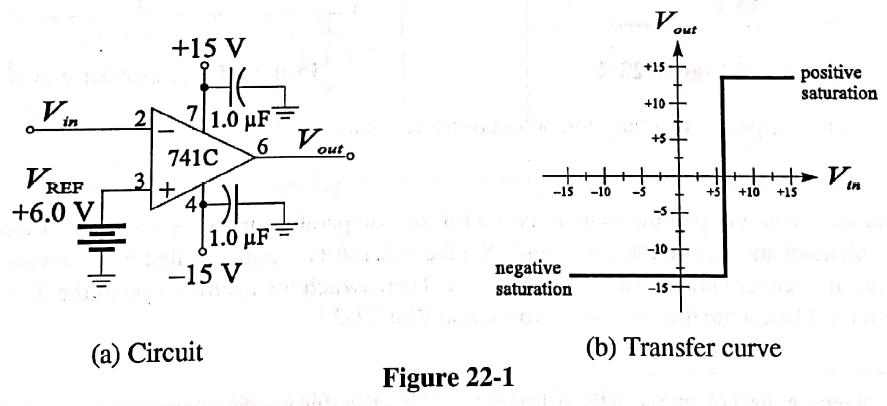
\includegraphics[width=0.95\textwidth]{figs/fig22-1.png}
\caption{Comparator circuit (a) and its transfer curve (b)}
\label{fig:22-1}
\end{figure}

Because of the sensitivity to a small input change, the output of a comparator may change due to noise on the input or when the input changes slowly. To avoid this, hysteresis is added to the comparator circuit by introducing positive feedback. The circuit, called a \textit{Schmitt trigger}, has two switching thresholds -- one for a rising input voltage, the other for a falling input. By separating the two thresholds, noise effects can be eliminated. In this experiment, you will investigate two comparators and an inverting Schmitt trigger circuit.

\newpage
% =====================================================
% PROCEDURE
% =====================================================
\section*{Procedure}

\subsection*{Comparator and Comparator Transfer Curve}

\begin{enumerate}[label=\arabic*.]
    \item Figure~\ref{fig:22-2} shows an inverting comparator circuit with a variable threshold determined by the potentiometer setting. Construct the circuit and set $V_{REF}$ to near $0\,\text{V}$. Set the function generator for a $3\,V_{pp}$ triangle waveform at $50\,\text{Hz}$ and observe the input and output waveforms on a two-channel oscilloscope. Sketch the waveforms on Plot 22-1. Note the point where switching takes place. Be sure to label all plots in this experiment.
\end{enumerate}

\begin{figure}[h!]
\centering
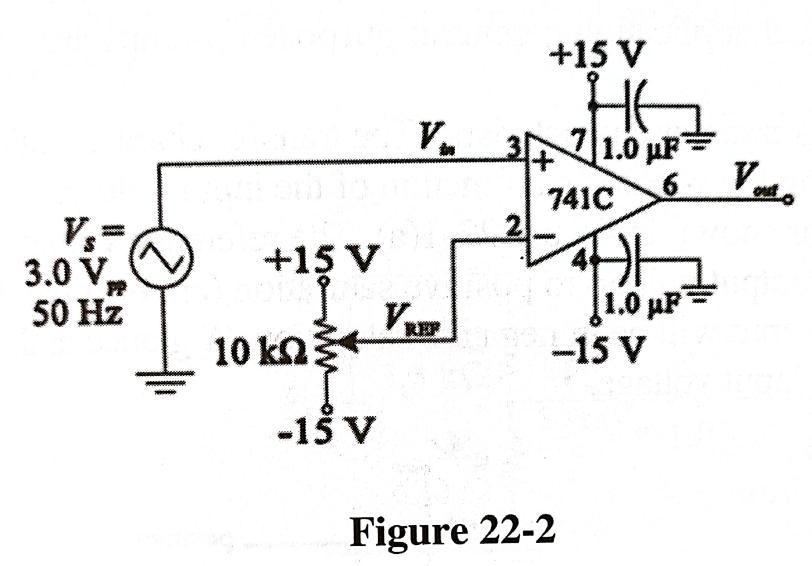
\includegraphics[width=0.55\textwidth]{figs/fig22-2.png}
\caption{Inverting comparator with variable threshold}
\label{fig:22-2}
\end{figure}

\begin{figure}[H]
\centering
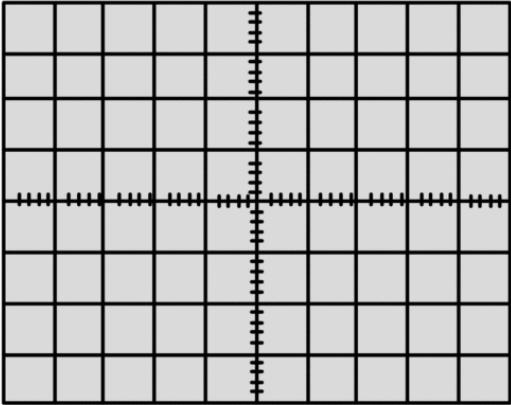
\includegraphics[width=0.55\textwidth]{figs/grid.png}
\caption{Plot 22-1 --- Comparator waveform.}
\label{plot:22-1}
\end{figure}

\begin{enumerate}[resume, label=\arabic*.]
    \item Observe the output as you vary the potentiometer. Then reset $V_{REF}$ to $0\,\text{V}$.

    Observations: \blank{10cm}.

    \item In this step, you will plot the transfer curve for the comparator on the oscilloscope. Place $V_{in}$ on the X-channel and $V_{out}$ on the Y-channel. Set the \textit{VOLTS/DIV} control so that both signals are on the screen. Neither channel should be inverted. Then switch the oscilloscope to the X-Y mode. Sketch (and label) the transfer curve you see in Plot 22-2.
\end{enumerate}

\begin{figure}[H]
\centering
\begin{minipage}{0.48\textwidth}
\centering
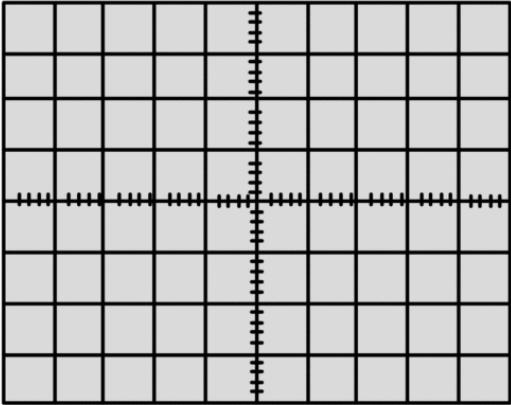
\includegraphics[width=\textwidth]{figs/grid.png}
\caption{Plot 22-2 --- Comparator transfer curve.}
\label{plot:22-2}
\end{minipage}
\hfill
\begin{minipage}{0.48\textwidth}
\centering
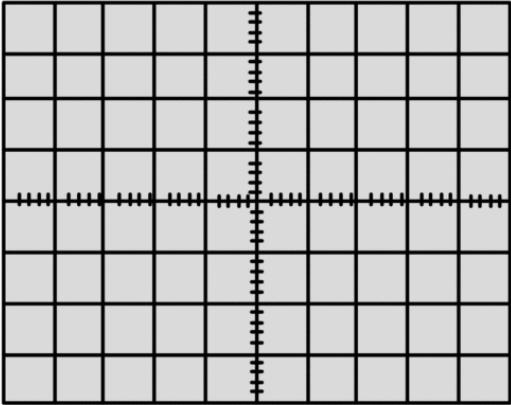
\includegraphics[width=\textwidth]{figs/grid.png}
\caption{Plot 22-3 --- Comparator transfer curve (inputs reversed).}
\label{plot:22-3}
\end{minipage}
\end{figure}

\begin{enumerate}[resume, label=\arabic*.]
    \item Vary the potentiometer as you observe the transfer curve.

    Observations: \blank{10cm}

    \blank{16cm}

    \item While observing the transfer curve, reverse the inputs to the comparator. Sketch the new transfer curve in Plot 22-3.
\end{enumerate}

\subsection*{Schmitt Trigger and Schmitt Trigger Transfer curve}

\begin{enumerate}[resume, label=\arabic*.]
    \item Construct the Schmitt trigger circuit shown in Figure~\ref{fig:22-3}. Set the potentiometer to the maximum resistance and put the oscilloscope in normal time base mode (not X-Y mode). Slowly reduce the resistance of the potentiometer and observe the input and output waveforms. Note that when the output changes states, the input voltage is different for a rising and a falling signal. Sketch the observed input and output waveforms in Plot 22-4.
\end{enumerate}

\begin{figure}[h!]
\centering
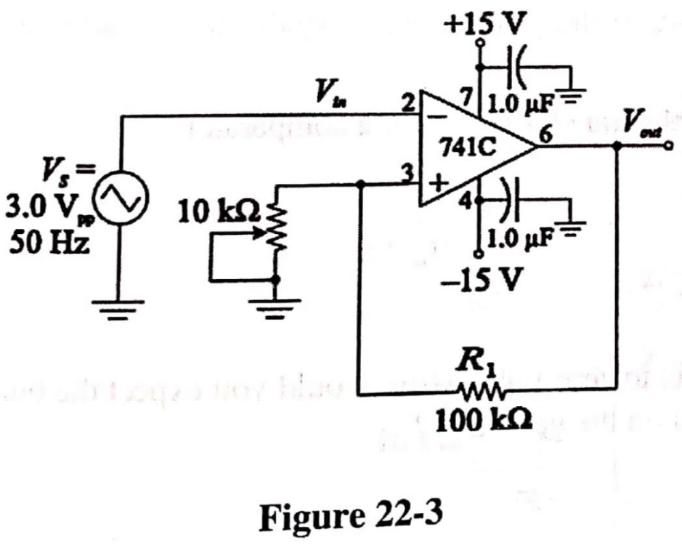
\includegraphics[width=0.5\textwidth]{figs/fig22-3.png}
\caption{Inverting Schmitt trigger circuit}
\label{fig:22-3}
\end{figure}

\begin{figure}[H]
\centering
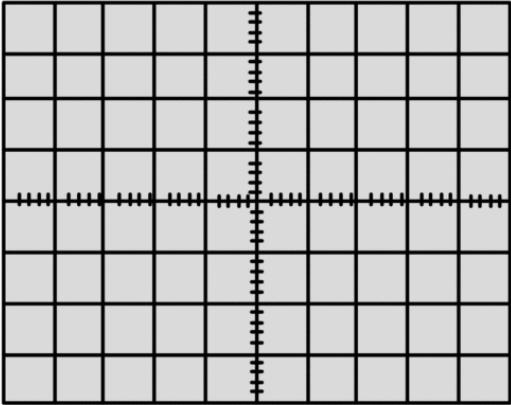
\includegraphics[width=0.55\textwidth]{figs/grid.png}
\caption{Plot 22-4 --- Schmitt trigger waveform.}
\label{plot:22-4}
\end{figure}

\newpage

\begin{enumerate}[resume, label=\arabic*.]
    \item In this step, you will plot the transfer curve for the Schmitt trigger on the oscilloscope. The input signal is again on the X-channel and the output signal is on the Y-channel. Select the X-Y mode and adjust the controls to view the transfer curve. Notice the hysteresis. Sketch (and label) the transfer curve you see in Plot 22-5.

    \item While observing the transfer curve, vary the potentiometer.

    Observations: \blank{10cm}

    \blank{16cm}
\end{enumerate}

\begin{figure}[H]
\centering
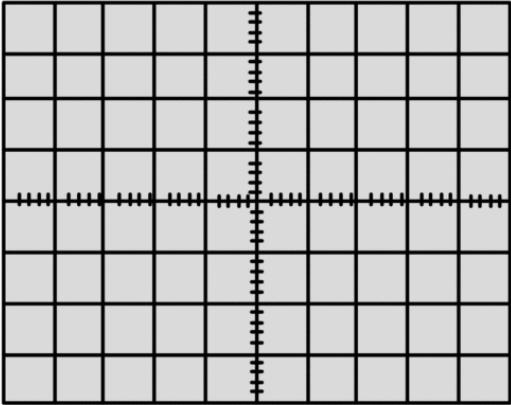
\includegraphics[width=0.55\textwidth]{figs/grid.png}
\caption{Plot 22-5 --- Schmitt trigger transfer curve.}
\label{plot:22-5}
\end{figure}

\newpage
% =====================================================
% CONCLUSION
% =====================================================
\section*{Conclusion}

Con el comparador de la Figura~\ref{fig:22-2} se vio que la salida del 741C solo tiene dos estados útiles y que el paso de uno al otro ocurre justo cuando $V_{in}$ cruza a $V_{REF}$. Como la triangular entra por el pin 3, la salida se va a saturación positiva mientras $V_{in} > V_{REF}$, entonces el circuito se comporta como un comparador no inversor aunque el enunciado lo llame inversor. En modo X-Y eso aparece como un escalón vertical, y al mover el potenciómetro ese escalón se corre a lo largo del eje de $V_{in}$ sin cambiar de forma. Con el umbral cerca de $+1.4\,\text{V}$ la salida pasó casi todo el ciclo en negativo y solo subía en los picos de la triangular, y con el umbral cerca de $-1.2\,\text{V}$ pasó lo contrario. O sea, el comparador convierte la triangular en una cuadrada cuyo ciclo de trabajo se controla con $V_{REF}$.

La saturación del 741C tampoco salió simétrica. En las capturas el nivel alto quedó alrededor de $+10.5\,\text{V}$ y el bajo alrededor de $-14.7\,\text{V}$, por eso no conviene asumir los $\pm 13\,\text{V}$ del libro sin medirlos antes.

En el Schmitt trigger de la Figura~\ref{fig:22-3} la realimentación positiva a través de $R_1$ y el potenciómetro separa el umbral de subida del de bajada, con
\[
V_{UT} = V_{sat+}\,\frac{R_{pot}}{R_{pot}+R_1}, \qquad V_{LT} = V_{sat-}\,\frac{R_{pot}}{R_{pot}+R_1}
\]
Con el potenciómetro al máximo la salida bajó cuando la entrada subía por $+0.95\,\text{V}$ y volvió a subir cuando la entrada bajaba por $-1.4\,\text{V}$, bastante cerca de lo que da la ecuación con los niveles de saturación medidos ($+0.95\,\text{V}$ y $-1.34\,\text{V}$). Los umbrales quedaron asimétricos por la misma razón que la salida. En X-Y la curva se abre en un lazo rectangular, más ancho con el potenciómetro al máximo, y al bajar la resistencia se va cerrando hasta desaparecer, punto en el que el circuito queda como un comparador simple con umbral en $0\,\text{V}$. Eso sí, $V_{LT}$ quedó muy cerca del mínimo de la triangular, y con una señal un poco más pequeña la salida se habría quedado trabada en saturación negativa.

La diferencia práctica entre los dos circuitos está en lo que pasa cerca del umbral. El comparador simple cambia de estado con cualquier variación alrededor de $V_{REF}$, mientras que el Schmitt trigger necesita que la entrada recorra todo el ancho de la histéresis antes de volver a cambiar, y eso lo hace inmune a cualquier ruido más pequeño que esa ventana, que en este montaje era de unos $2.3\,\text{V}$.

\vspace{9cm}

\newpage
% =====================================================
% EVALUATION AND REVIEW QUESTIONS
% =====================================================
\section*{Evaluation and Review Questions}

\begin{enumerate}[label=\arabic*.]
    \item Describe how the threshold voltage changes the transfer curve for a comparator.

    \vspace{2.5cm}

    \item Assume the circuit in Figure~\ref{fig:22-2} had $V_{REF}$ set to zero volts. How would you expect the output to be affected by varying the dc offset control on the generator?

    \vspace{2.5cm}

    \item Would a sinusoidal input to the comparators produce the same transfer curve as a triangle waveform? Explain.

    \vspace{2.5cm}

    \item Summarize the important differences between a comparator and Schmitt trigger.

    \vspace{2.5cm}

    \item Assume the input signal in Figure~\ref{fig:22-3} could have as much as $100\,\text{m}V_{pp}$ noise. To avoid multiple tripping due to noise, you need to set the trip points at least $100\,\text{mV}$ apart. What is the minimum value of resistance that the potentiometer can be set? Assume the output saturates at $\pm 13\,\text{V}$.

    \vspace{2.5cm}
\end{enumerate}

\newpage
% =====================================================
% FOR FURTHER INVESTIGATION
% =====================================================
\section*{For Further Investigation}

The Schmitt trigger you investigated in the experiment can be modified slightly to form a relaxation oscillator. Investigate the relaxation oscillator shown in Figure~\ref{fig:22-4}. (For simplicity, power supply connections are not shown.) Look at the waveform across the capacitor and at the output. Test the effect of the potentiometer on the frequency and waveform on the capacitor. Normally, a triangle waveform is observed. Under what conditions can you obtain a sine wave? Then observe the transfer curve by observing the signal on pin 2 and pin 6 in the X-Y mode, can you explain the shape? Summarize your findings in a short report.

\begin{figure}[h!]
\centering
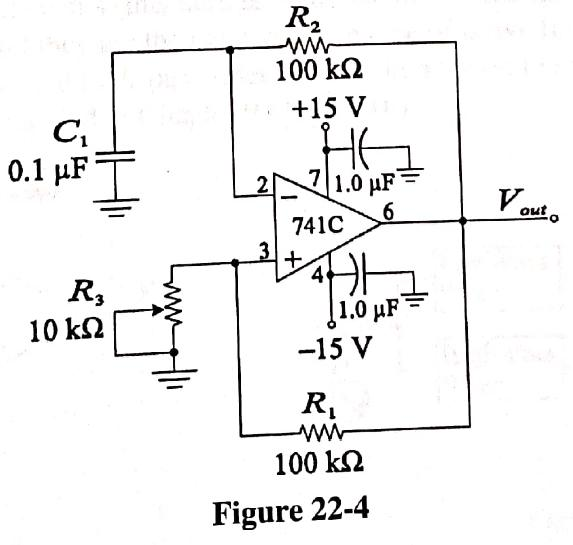
\includegraphics[width=0.5\textwidth]{figs/fig22-4.png}
\caption{Relaxation oscillator based on the Schmitt trigger}
\label{fig:22-4}
\end{figure}

\end{document}
